\section{Task Assignment}

One of the many benefits of a decentralized multi-agent algorithm is the ability to decompose a problem into parallelizable components.  In order to realize the full potential of a distributed multi-agent algorithm, a cooperative approach that coordinates tasks in a non-overlapping manner becomes necessary.  The Cooperative Assignment of Swarm Tasks (CAST) auction \cite{palmer:CAST} is a fully decentralized task assignment algorithm based on synchronized random number generators that requires only agent-local knowledge about all possible tasks.  The CAST auction exhibits several desirable features for a swarm including parallel computations, a limited number of broadcast communications, workable solutions with very short computations, and  additional solution refinement with increased computation time.  In addition, the CAST auction guarantees that with enough time the optimal solution will be found.

The basic assumptions of the CAST auction algorithm are minimal.  First, assume that each agent has a random number generator that can be synchronized across the swarm.  This can be done by broadcasting a common seed or having a common list of seeds ready for use.  The CAST auction also requires that all agents can perform a broadcast communication that all other members of the swarm can receive.  In addition, assume that all agents either have or can compute their cost for each task.

The basic principle of the CAST auction is a time-limited, probabilistic search of the full permutation space that yields good solutions with comparatively small amounts of computation and communication.  The steps of this approach are as follows:

\begin{enumerate}
\item All agents compute their cost tables for the task independently.

\item  Agents sort their choice lists in descending order of task cost.
  
\item Each agent internally computes the bid order for the current round of bidding.
  
\item \label{bid} The current bidder selects their best choice task and broadcasts the selected task and associated. 
  
\item On receiving a broadcasted selection, the selected task is removed from the task pool and the task cost is added to the accumulated cost for this round.
  
\item If the end of a round is not reach, goto \ref{bid}, else \ref{finish}.
  
\item \label{finish} Repeat the auction with a different bid order as needed.  If the cost is less, the new task mapping is adopted.
\end{enumerate}

\refTable{CastParameters} is a summary of the simulation parameters used in implementing the CAST auction algorithm.  Each agent is capable of two actions, \emph{Receive-Bid} which listens for a bid broadcast, and \emph{Bid} which selects the best task available with respect to the bidding agent's preferences and broadcasts that choice.  Each agent is able to determine if it is their turn to bid through the binary sensor \emph{Is-Turn-To-Bid} which returns true if it is the agent's turn to bid and false otherwise.

\begin{table}[ht]
  \centering
  \begin{tabular}{|l|l|}
    \hline
    \textbf{Number of Agents} & 10, 50 \\
    \hline
    \textbf{Number of Tasks} & 10, 50 \\
    \hline
    \textbf{Number of Rounds} & 1, 10, 50, 100 \\
    \hline
    \textbf{Actions} & Bid-on-Task \\
    \hline
    \textbf{Task Evaluation Criteria} & Cartesian distance \\
    \hline
  \end{tabular}
	
  \caption{Summary of CAST Auction simulation parameters}
  \label{tab:CastParameters}
\end{table}

\begin{figure}[ht]
	\centering
	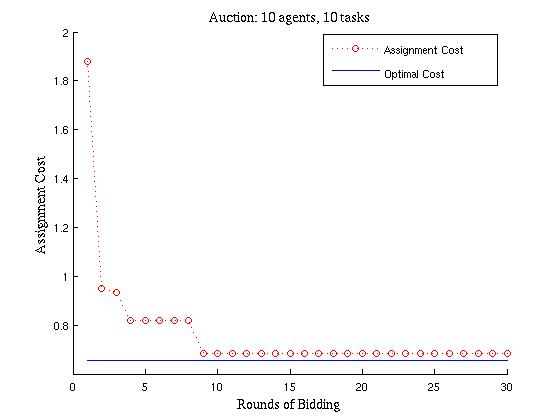
\includegraphics[scale=.65]{Figures/CAST_10.jpg}
\caption[Results from an example CAST auction.]{Results from a CAST auction with 10 agents, 10 tasks, and costs in the range of $(0,1)$.  Notice that the CAST auction quickly finds a near-optimal solution.}
\label{fig:Cast10}
\end{figure}

In order to compare results to those found in \cite{palmer:CAST}, assignments with 10 agents and 10 tasks are simulated.  For each instance of the problem, the position of both the agents and the tasks were randomized.  \refFigure{Cast10} shows the results from one run of the CAST auction with 10 agents, 10 tasks, and each task having a cost in the range of $(0,1)$.  The optimal assignment, as computed through brute force, has a total cost of 0.6423.  In round 9, the CAST auction finds an assignment with a total cost of 0.6557, with successive rounds of auctioning producing no further progress.  The results of the CAST auction implementation are consistent with the results found in \cite{palmer:CAST}, with near-optimal solutions (within 90\%) being found within 10 bidding rounds.  


